\labeledsection{Markov Decision Processes}{sec:mdp}
\centeredtitledbox{Motivation}{
In \linkterm{deterministic}{env_types} environments, the next state is completely determined by the current state and the chosen action. For these problems, we define a corresponding \linkterm{deterministic}{env_types} \linkterm{search problem}{search_problem} where the objective is to find a \linkterm{solution}{search_prob_sol} consisting of a specific \linkterm{sequence}{sequence} of actions—an optimal plan—leading from the initial state to a goal state.

However, in a \linkterm{stochastic}{env_types} environment, the next state is \textbf{not} uniquely determined by the current state and action. In these \linkterm{stochastic}{env_types} \linkterm{search problems}{search_problem}, the \linkterm{agent}{def:agent} controls the action but lacks direct control over the environment's transitions. While the exact outcome of an action is unknown, the \linkterm{agent}{def:agent} knows the probabilities of transitioning to various states given a specific action.

Consequently, a fixed \linkterm{sequence}{sequence} of actions is no longer sufficient. Instead, the goal is to find an \textbf{optimal policy}, $\pi^{*}$, which is a \linkterm{function}{function} $\pi^{*}: \mathcal{S} \to \mathcal{A}$ that dictates the best action for any given state. By following this policy, the \linkterm{agent}{def:agent} navigates the environment's uncertainty to reach a goal state efficiently.
}

\Example{
Consider a grid world where the agent can go west, east, north, or south. Notice the difference between \linkterm{deterministic}{env_types} and \linkterm{stochastic}{env_types} environments:

\begin{figure}[H]
    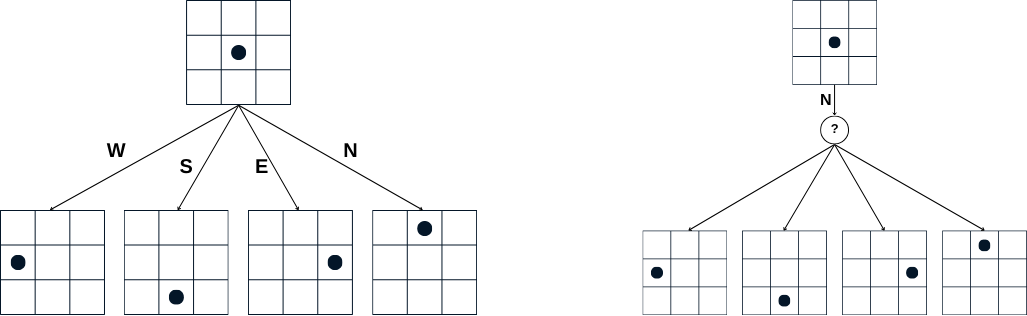
\includegraphics[width=\linewidth]{images/deterministic_vs_stochastic.png}
\end{figure}
}{}

\commandnote{
We are still assuming \linkterm{fully observable}{env_types} environments
}

\definition{MDP Running Example}{
We will consider the following \linkterm{fully observable}{env_types} $4 \times 3$ grid world with \linkterm{stochastic}{env_types} actions:

\begin{figure}[H]
    \centering
    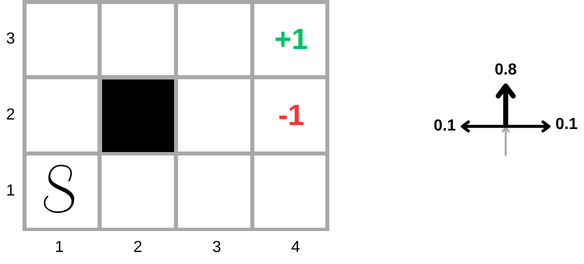
\includegraphics[width=0.4\linewidth]{images/mdp_running_ex.png}
\end{figure}
}{mdp_running_ex}

\definition{MDP}{
A \defemph{Markov Decision Process (MDP)} is the \linkterm{structure}{def:math_structure} $\tuple{\mathcal{S}, \mathcal{A}, \mathcal{T}, \mathcal{I}, R}$ where:
\begin{itemize}
    \item $\mathcal{S}$: the \linkterm{set}{def:set} of states
    \item $\mathcal{I}$: the \linkterm{set}{def:set} of initial states. Since we are in a \linkterm{fully observable}{env_types} environment, $\mathcal{I}=\set{s_0}$.
    \item $\mathcal{A}$: the \linkterm{set}{def:set} of actions, with $\mathcal{A}_s$ denoting the \linkterm{set}{def:set} of action that can be taken from state $s$.
    \item $\mathcal{T}$: a transition model $\mathcal{T}(s,a)=\probd{\mathcal{S}\mid s, a}$
    \item $R$: a \defemph{reward function} $\func{R}{\mathcal{S}}{\mathbb{R}}$ \hfill (we call $R(s)$ a \defemph{reward})
\end{itemize} 
}{MDP}

\ideabox{
We use the \linkterm{rewards}{MDP} as a utility function: the goal is to choose actions such that the expected comulative \linkterm{rewards}{MDP} for the foreseeable future is maximized.
}

\commandnote{
In \linkterm{MDPs}{MDP}, the aim is to find an \textbf{optimal policy} $\pi(s)$, which tells us the best action for every possible state $s$. (because we can't predict where we might end up, we need to consider all states)
}

\definition{Policy}{
A \defemph{policy} $\pi$ for an \linkterm{MDP}{MDP} is a \linkterm{function}{function} mapping each state $s \in \mathcal{S}$ to an action $a \in \mathcal{A}_s$. An \defemph{optimal policy} is a policy that maximizes the expected total \linkterm{rewards}{MDP}.
}{policy}

\Example{
\begin{figure}[H]
     \centering
     \begin{subfigure}[b]{0.24\textwidth}
         \centering
         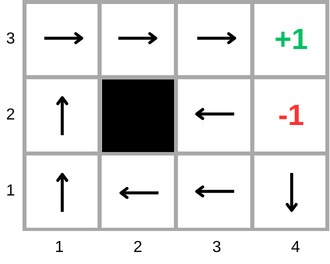
\includegraphics[width=\textwidth]{images/reward-0.01.png}
         \caption{$R(s) = -0.01$}
         \label{fig:sub1}
     \end{subfigure}
     \hfill
     \begin{subfigure}[b]{0.24\textwidth}
         \centering
         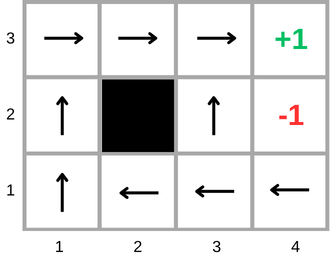
\includegraphics[width=\textwidth]{images/reward-0.03.png}
         \caption{$R(s) = -0.03$}
         \label{fig:sub2}
     \end{subfigure}
     \hfill
     \begin{subfigure}[b]{0.24\textwidth}
         \centering
         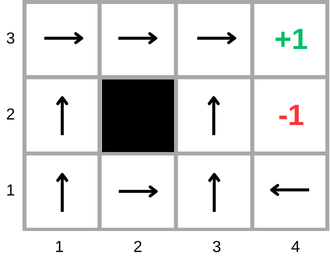
\includegraphics[width=\textwidth]{images/reward-0.4.png}
         \caption{$R(s) = -0.4$}
         \label{fig:sub3}
     \end{subfigure}
     \hfill
     \begin{subfigure}[b]{0.24\textwidth}
         \centering
         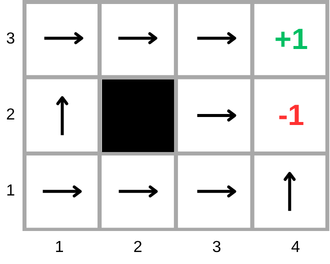
\includegraphics[width=\textwidth]{images/reward-2.png}
         \caption{$R(s) = -2$}
         \label{fig:sub4}
     \end{subfigure}
     \caption{Different optimal policies for different reward functions}
     \label{fig:policy_vs_reward_ex}
\end{figure}

For $R(s) = -0.01$, we have a small negative reward for each state. Hence, each action will cost a little bit and not too much. Therefore, in state $(3,2)$, the optimal action is to go west where there is a $80\%$ chance we stay where we are. We cannot go north since there is a $10\%$ of ending up in the pit ($-1$). Because the action costs only $0.01$, the agent prefers to bang his head to the wall until by chance goes north or south. Similarly, in $(4,1)$.

For $R(s) = -0.03$, the action cost is a bit high. The agent prefer to take the chance of going north (in $(3,2)$) and west in $(4,1)$ regardless of the $10\%$ probability of falling in the pit. 

For $R(s) = -0.4$, the cost now is much higher, the agent will try to finish as soon as possible.

For $R(s) = -2$, life is very painful, the agent might commit suicide to alleviate the pain.
}{}

\questionbox{
Assume we have two sequences of three actions, the first one will collect the rewards $1,2,2$, and second one will collect $2,3,4$. Which sequence should the agent choose?
}

\answerbox{
Well, since we agreed that we want to maximize the total sum of rewards, obviously we should prefer $2,3,4$ because they sum to $9>5$.
}

\questionbox{
What about $0,0,1$ and $1,0,0$?
}

\observationbox{
They have the same total sum of rewards.
}

\ideabox{
\begin{itemize}
    \item It is reasonable to maximize the sum of rewards
    \item But it is also reasonable to prefer rewards \textbf{now} over rewards \textbf{later}
\end{itemize}
}

\answerbox{
Then the agent should prefer $1,0,0$ over $0,0,1$
}

\questionbox{
But how can we model this into the agent's brain?
}

\answerbox{
We should let the values of the rewards decay exponentially over time
}

\anondefinition{
We call \linkterm{preferences}{preferences} on \linkterm{reward}{MDP} \linkterm{sequences}{sequence} \defemph{stationary} iff
\[
[r, r_0, r_1, r_2, \cdots] \succ [r, r'_0, r'_1, r'_2, \cdots] \Leftrightarrow [r_0, r_1, r_2, \cdots] \succ [r'_0, r'_1, r'_2, \cdots]
\]
}{stationary_preferences}

\Theorem{
For \linkterm{stationary preferences}{stationary_preferences}, there are only two ways to combine \linkterm{rewards}{MDP} over time:
\begin{itemize}
    \item \defemph{additive rewards}: $U([s_0, s_1, s_2, \cdots]) = R(s_0) + R(s_1) + R(s_2) + \cdots$
    \item \defemph{discounted rewards}: $U([s_0, s_1, s_2, \cdots]) = R(s_0) + \gamma R(s_1) + \gamma^2 R(s_2) + \cdots$ where $0 \leq \gamma \leq 1$ is called \defemph{discount factor}
\end{itemize}
}{discounted_rewards}

\questionbox{
Given \linkterm{discounted rewards}{discounted_rewards} with $\gamma=0.5$, what is the utility of the \linkterm{rewards}{MDP} \linkterm{sequences}{sequence} $[1,2,3]$, and $[3,2,1]$?
}

\answerbox{
\begin{itemize}
    \item $U([1,2,3]) = 1 + 0.5 \cdot 2 + 0.25 \cdot 3 = 2.75$
    \item $U([3,2,1]) = 3 + 0.5 \cdot 2 + 0.25 \cdot 1 = 4.25$
\end{itemize}

$U([3,2,1]) >  U([1,2,3])$ (the sooner the better)
}

\minititle{Dicounting Exercise}
Consider the following world:
\begin{figure}[H]
    \centering
    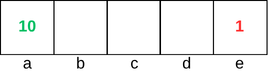
\includegraphics[width=0.2\linewidth]{images/abcde.png}
\end{figure}
\begin{itemize}
    \item $\mathcal{S}=\set{a,b,c,d,e}$
    \item $\mathcal{A}_s = \set{E,W} \quad \forall s \in \set{b,c,d}$ \hfill(East and West)
    \item $\mathcal{T}$ is \linkterm{deterministic}{env_types}
    \item If we are in $a$, we get \linkterm{reward}{MDP} $10$.
    \item If we are in $e$, we get \linkterm{reward}{MDP} $1$.
    \item $R(s)=0 \quad \forall s \in \set{b,c,d}$
\end{itemize}

\questionbox{
For $\gamma=1$ (no \linkterm{discounted rewards}{discounted_rewards}), what is the optimal policy ?
}

\answerbox{
\begin{figure}[H]
    \centering
    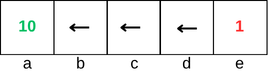
\includegraphics[width=0.2\linewidth]{images/abcde_1.png}
\end{figure}
}

\questionbox{
For $\gamma=0.1$, what is the optimal policy ?
}

\answerbox{
\begin{figure}[H]
    \centering
    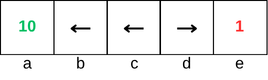
\includegraphics[width=0.2\linewidth]{images/abcde_2.png}
\end{figure}
}

\questionbox{
For which $\gamma$ are West and East equally good when agent in state $d$?
}

\answerbox{
\begin{itemize}
    \item Going East: $0+\gamma \cdot 1$
    \item Going West: $0 + \gamma \cdot 0 + \gamma^2 \cdot 0 + \gamma^3 \cdot 10$
    \item $\gamma = 10 \cdot \gamma^3$
    \item $1 = 10 \cdot \gamma^2$
    \item $\gamma^2 = \frac{1}{10} \leadsto \gamma = \frac{1}{\sqrt{10}}$
\end{itemize}
}

\redbox{
What if we do not have terminal states ?
}

\observationbox{
If we are using \linkterm{additive rewards}{discounted_rewards} and we do not have terminal states, we can get infinite reward!
}

\ideabox{
We have two solutions to this problem:
\begin{itemize}
    \item Finite Horizon: we terminate after a fixed $T$ steps. $\leadsto$ Gives \linkterm{non-stationary}{stationary_preferences} policies ($\pi$ depends on the time left)
    \item Absorbing States: for any policy $\pi$, the agent eventually dies with probability $=1$. $\leadsto$ \linkterm{Expected utility}{expected_utility} of every state is finite
\end{itemize}
}

\observationbox{
A better solution is to use \linkterm{discounted rewards}{discounted_rewards} with $0 \leq \gamma < 1$.
}

\Proof{
\begin{itemize}
\item Let $R_{\text{max}}$ be the maximum reward the agent can get.
\item $U([r_0, r_1, r_2, \cdots, r_{\infty}]) = \sum_{t=0}^{\infty} \gamma^t r_t$
\item $\sum_{t=0}^{\infty} \gamma^t r_t \leq \sum_{t=0}^{\infty} \gamma^t R_{\text{max}}$
\item $\sum_{t=0}^{\infty} \gamma^t R_{\text{max}}$ is a convergent geometric series (since $\gamma < 1$)
\item $\sum_{t=0}^{\infty} \gamma^t R_{\text{max}} = \frac{R_{\text{max}}}{1-\gamma}$
\item Therefore, $U([r_0, r_1, r_2, \cdots, r_{\infty}]) \leq \frac{R_{\text{max}}}{1-\gamma}$
\end{itemize}
}

\minititle{Remember - The Geometric Series}

\anondefinition{
A \textbf{geometric series} is the sum of an infinite sequence where each term is found by multiplying the previous one by a fixed, non-zero constant $r$, called the \textbf{common ratio}. Given an initial term $a \neq 0$, the series is expressed as:
\[ \sum_{n=0}^{\infty} ar^n = a + ar + ar^2 + ar^3 + \dots \]
}{}

To determine if the infinite sum exists, we define the \textbf{$k$-th partial sum}, $S_k$, as the sum of the first $k$ terms:
\[ S_k = \sum_{n=0}^{k-1} ar^n = a + ar + ar^2 + \dots + ar^{k-1} \]
Through algebraic manipulation, this can be written in closed form as:
\[ S_k = a \left( \frac{1-r^k}{1-r} \right) \quad \text{for } r \neq 1 \]


The infinite series converges if the limit of the partial sums exists and is finite:
\[ S = \lim_{k \to \infty} S_k \]

If the magnitude of the ratio is less than one ($|r| < 1$), then the term $r^k$ vanishes as $k$ approaches infinity:
\[ \lim_{k \to \infty} r^k = 0 \]

Substituting this into the partial sum formula yields the \textbf{sum of the infinite geometric series}:
\[ S = \lim_{k \to \infty} a \left( \frac{1-r^k}{1-r} \right) = a \left( \frac{1-0}{1-r} \right) = \frac{a}{1-r} \]

\begin{itemize}
    \item If \textbf{$|r| < 1$}, the series \textbf{converges} to $\frac{a}{1-r}$.
    \item If \textbf{$|r| \geq 1$}, the series \textbf{diverges} (the sum does not approach a finite limit).
\end{itemize}

\anondefinition{
Given a \linkterm{sequence}{sequence} of state $S=s_0, s_1, s_2, \cdots$ and a \linkterm{discount factor}{discounted_rewards} $0 \leq \gamma < 1$, the \defemph{utility} of the \linkterm{sequence}{sequence} is :
\[
U(S) = \sum_{t=0}^{\infty} \gamma^t R(s_t)
\]
}{utility_seq_states_mdp}

\anondefinition{
Given a \linkterm{policy}{policy} $\pi$ and a starting state $s_0$. We define a \linkterm{random variable}{def:random_variable} $S_{s_0}^{\pi}$ which represent the \linkterm{sequence}{sequence} of states resulting from executing $\pi$ at every state starting from $s_0$ (because the environment is \linkterm{stochastic}{env_types}, we do not know the exact sequence, hence the \linkterm{random variable}{def:random_variable} treatment).
}{state_sequence_rv}

\anondefinition{
The \defemph{expected utility} obtained by executing the policy $\pi$ starting in $s_0$ is given by:
\[
U^{\pi} (s_0) := \text{EU}(\linkterm{S_{s_0}^{\pi}}{state_sequence_rv})
\]
}{expected_utility_mdp}

\anondefinition{
The \defemph{optimal policy} $\pi^{*}$ is a policy that maximizes the \linkterm{expected utility}{expected_utility} for the agent:
\[
\pi^{*}_{s_0} := \argmax{\pi} U^{\pi} (s_0)
\]
}{optimal_policy_mdp}

\observationbox{
While we initially define it relative to a starting state $s_0$. It is a fundamental property of MDPs that there exists a single policy $\pi^{*}$ that is optimal for \textbf{all} starting states simultaneously.
}

\anondefinition{
The \defemph{true utility} $U(s)$ of a state is the \linkterm{expected utility}{expected_utility_mdp} obtained by following the \linkterm{optimal policy}{optimal_policy_mdp} starting in that state:
\[ U(s) = U^{\pi^{*}}(s) \]
}{state_utility_mdp}

\anondefinition{
Once these \linkterm{utilities}{state_utility_mdp} are known, the \linkterm{optimal policy}{optimal_policy_mdp} can be extracted locally using the \linkterm{MEU}{def:MEU} principle. Choosing the best action is just maximizing the \linkterm{expected utility}{expected_utility} of the immediate successor states:
\[
\pi^{*}(s) = \argmax{a \in \mathcal{A}_s} \left( \sum_{s'} P(s' \mid s, a) \cdot U(s') \right)
\]
}{optimal_action_mdp}

\Example{
Assume we know the \linkterm{utilities}{state_utility_mdp} of our grid world:
\begin{figure}[H]
    \centering
    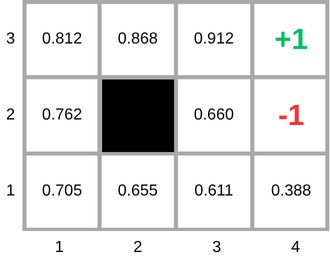
\includegraphics[width=0.3\linewidth]{images/mdp_running_ex_with_utilities.png}
\end{figure}

What is the \linkterm{optimal action}{optimal_action_mdp} for state $(3,4)$?

\begin{align*}
\pi^{*}(s) &= \argmax{a \in \mathcal{A}_s} \left( \sum_{s'} P(s' \mid s, a) \cdot U(s') \right) \\
\pi^{*}((3,4)) &= \argmax{a \in \set{\text{N, S, E, W}}} \left( \sum_{s'} P(s' \mid s, a) \cdot U(s') \right)
\end{align*}

For $a=N$, we have $s' \in \set{(3,2), (4,1), (2,1)}$
\[
\sum_{s'} P(s' \mid s, a) \cdot U(s') = 0.8 \cdot 0.660 + 0.1 \cdot 0.388 + 0.1 \cdot 0.655 = 0.6326
\]

For $a=S$
\[
\sum_{s'} P(s' \mid s, a) \cdot U(s') = 0.8 \cdot 0.611 + 0.1 \cdot 0.388 + 0.1 \cdot 0.655 = 0.5931
\]

For $a=E$
\[
\sum_{s'} P(s' \mid s, a) \cdot U(s') = 0.8 \cdot 0.388 + 0.1 \cdot 0.660 + 0.1 \cdot 0.611 = 0.4375
\]

For $a=W$
\[
\sum_{s'} P(s' \mid s, a) \cdot U(s') = 0.8 \cdot 0.655 + 0.1 \cdot 0.611 + 0.1 \cdot 0.660  = 0.6511
\]

Therefore:
\begin{align*}
\pi^{*}((3,4)) &= \argmax{a \in \set{\text{N, S, E, W}}} \left( \sum_{s'} P(s' \mid s, a) \cdot U(s') \right) = W
\end{align*}
}{}